%%%%%%%%%%%%%%%%%%%%%%%%%%%%%%%%%%%%%%%%%%%%%%%%%%%%%%%%%%%%%%%%%
% Qualificacao de Doutorado / Dept Fisica, CFM, UFSC            %
% Eduardo@UFSC - 2015                                           %
%%%%%%%%%%%%%%%%%%%%%%%%%%%%%%%%%%%%%%%%%%%%%%%%%%%%%%%%%%%%%%%%%

%:::::::::::::::::::::::::::::::::::::::::::::::::::::::::::::::%
%                                                               %
%                          Capítulo 4                           %
%                                                               %
%:::::::::::::::::::::::::::::::::::::::::::::::::::::::::::::::%

%***************************************************************%
%                                                               %
%                     Comparação SFR EML                        %
%                                                               %
%***************************************************************%

\chapter{Comparações entre propriedades estelares e propriedades nebulares}
\label{sec:synvsneb}

Precisamos entender as diferenças entre as propriedades que obtemos através da síntese espectral e
aquelas calculadas com as linhas de emissão. As propriedades da síntese são relacionadas às
populações estelares e comparações com as nebulares podem nos ajudar a entender melhor a história de
formação estelar de cada região. Durante os últimos anos esses estudos cruzados entre propriedades
sintéticas e nebulares de quase um milhão de galáxias do \SDSS renderam ótimos resultados para o
GAS-UFSC. Nesse capítulo faremos esse tipo de comparação utilizando as propriedades mais importantes
diretamente para a conversão de poeira em gás: taxa de formação estelar, coeficiente de extinção por
poeira e metalicidade.

\section{Comparação entre as taxas de formação estelar}
\label{sec:synvsneb:SFR}

Com a síntese de populações estelares podemos calcular a história de formação estelar utilizando o
vetor cumulativo de massa ($\eta_\star(t_\star)$), que integra a fração total de massa convertida em
estrelas para cada idade das populações da base ($\mu_j$). Então podemos calcular uma taxa de
formação dentro de um intervalo de tempo:
\begin{eqnarray}
	\eta_\star(t_\star)\ &=&\ \sum\limits_{t_{\star,j} < t_\star} \mu_j \\
	\overline{\mathrm{SFR}_\star}(t_\star)\ &=&\ M_\star \frac{(1\ -\ \eta_\star(t_\star))}{t_\star},
	\label{eq:SFRSyn}
\end{eqnarray}
\noindent onde $M_\star$ é a massa total convertida em estrelas durante toda a história de
formação estelar de uma galáxia. 

\begin{figure}
	\centering
	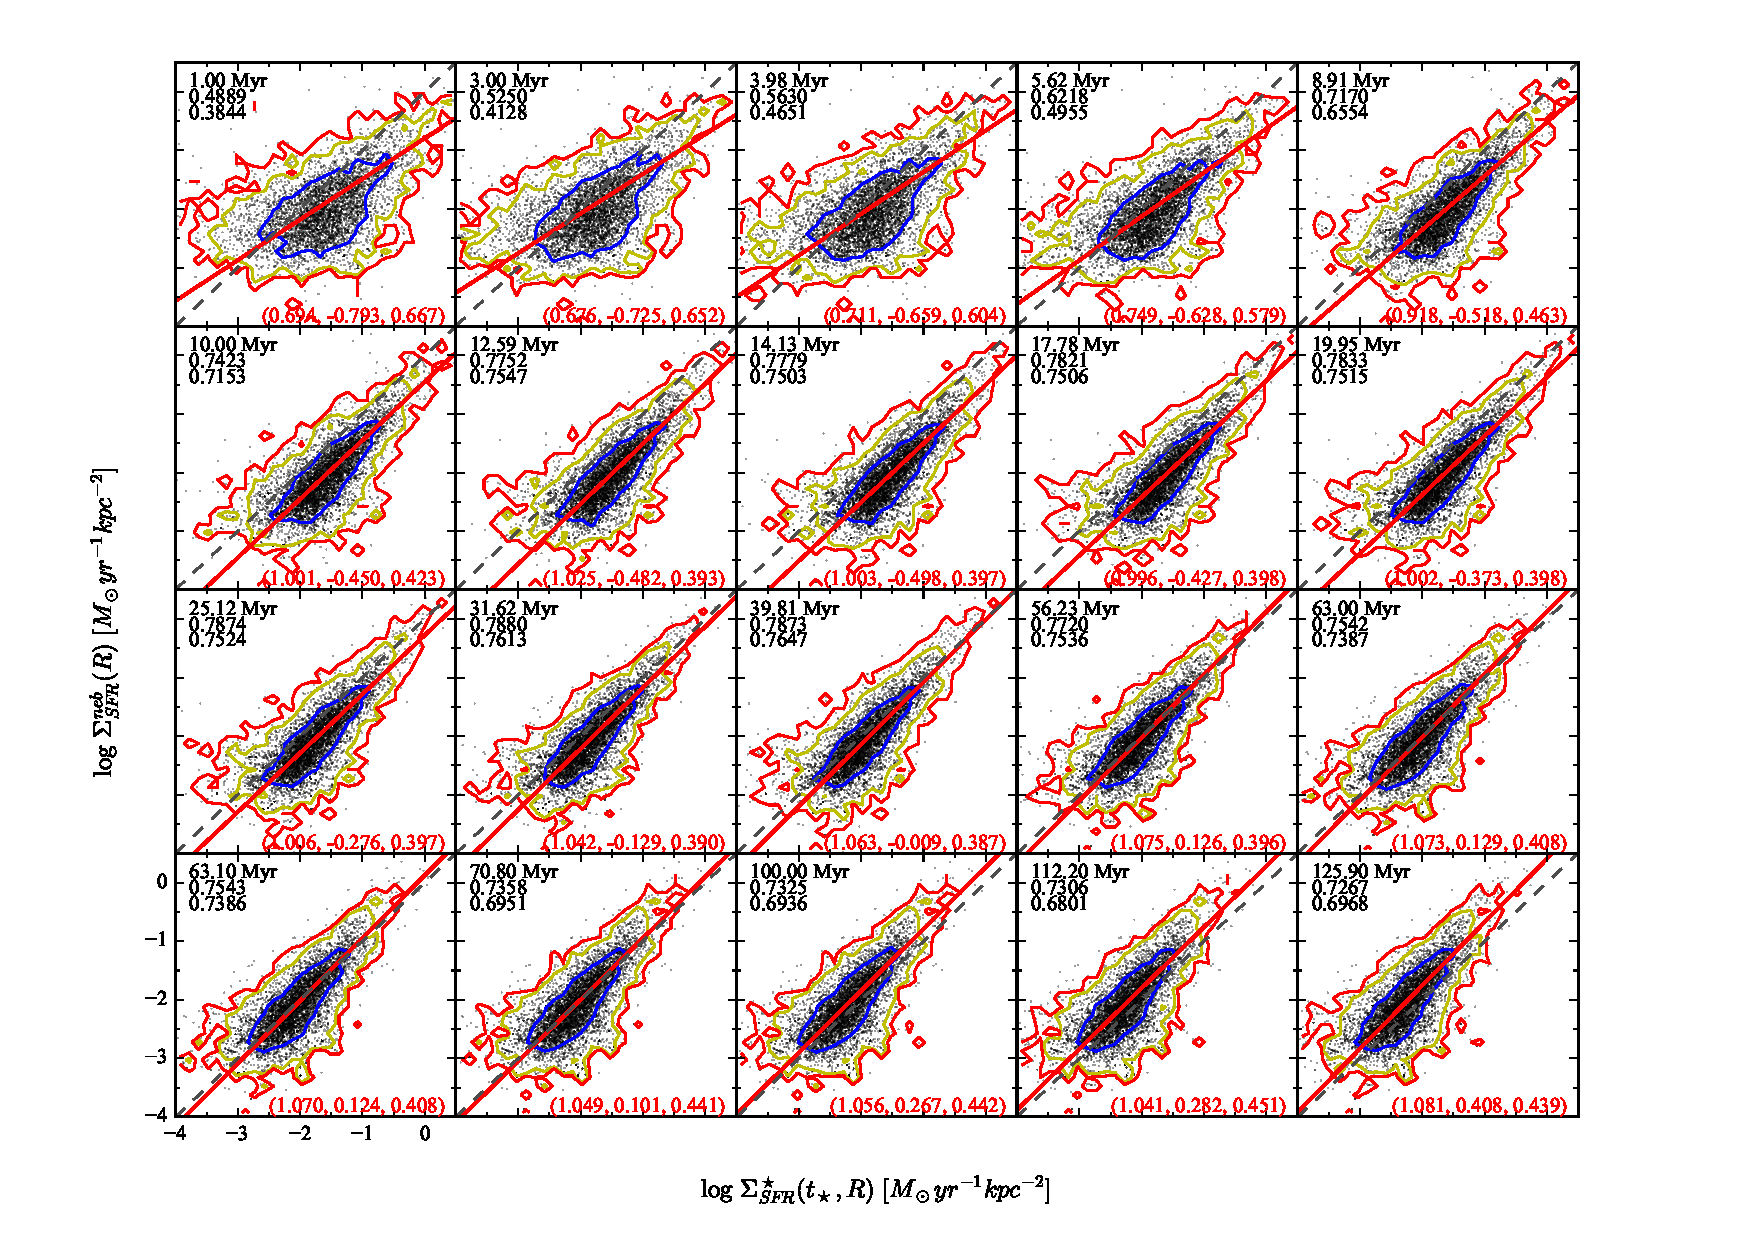
\includegraphics[scale=0.7, clip, angle=90]{figuras/aSFRSD_report.pdf}
	\caption[Comparação entre $\SigmaSFR$ e $\SigmaSFRN$ em {\em bins} radiais para diversas idades.]
	{comparação das duas densidades superficiais da taxa de formação estelar em {\em bins} radiais,
para diferentes valores de $t_\star$. Em cada gráfico temos os contornos em 1$\sigma$ (azul),
2$\sigma$ (verde) e 3$\sigma$ (vermelho) da distribuição. A linha vermelha indica o ajuste {\em OLS
bisector}, e os números em vermelho são o coeficiente angular, o ponto de interceptação com o eixo
$x$ e o valor $rms$ em torno do ajuste. No canto superior esquerdo está indicado $t_\star$, o
coeficiente de correlação de Spearmann e o de Pearson.}
	\label{fig:aSFRSDsynvsaSFRSDneb}
\end{figure}

Como explicado na Sec. \ref{sec:emlines:SFR}, podemos medir a taxa de formação estelar recente
medindo a luminosidade intrínseca de \Halpha. Com as duas taxas de formação estelar, uma referente
às estrelas com idade menor que 10 milhões de anos e estimada pela linha de emissão de \Halpha
\eqref{eq:SFRNeb}, outra proveniente da síntese de populações estelares, que pode ser avaliada em
diferentes tempos $t_\star$ em \eqref{eq:SFRSyn}. Geramos diversas figuras como a Fig.
\ref{fig:aSFRSDsynvsaSFRSDneb} para encontrar a idade que melhor relaciona as duas medidas (aqui a
chamamos de $t_{SF}$). Em todos os painéis vemos a comparação das duas densidades superficiais da
taxa de formação estelar, em {\em bins} radiais, para diferentes valores de $t_\star$, além de um
ajuste {\em OLS bisector} e os coeficiente de correlação de Spearmann e Pearson (números abaixo da
idade no canto superior esquerdo). Neste gráfico há apenas os cortes removendo as zonas aonde não há
S/N suficiente nas quatro linhas do BPT. Vemos que entre 12 e 56 milhões de anos o coeficiente de
correlação quase não muda, chegando ao máximo (0.7880 em 31.62 milhões de anos), ou seja, não há
muita diferença escolher idades neste intervalo nessa amostra, portanto escolhemos $t_{SF} = 31.62$
milhões de anos. Escolhemos fazer este tipo de análise utilizando as correlações entre densidades
superficiais pois são mais confiáveis já que removem o termo $d^2$ existente no cálculo da SFR, que
induz uma correlação direta entre $\mathrm{SFR}_\star$ e $\mathrm{SFR}_{\Halpha}$. Esse valor
de $t_{SF}$ não está muito distante da escala de tempo de vida das estrelas que produzem a
maioria dos fótons capazes de produzirem a linha de \Halpha ($\sim10^7$ anos).

\begin{figure}
	\centering
	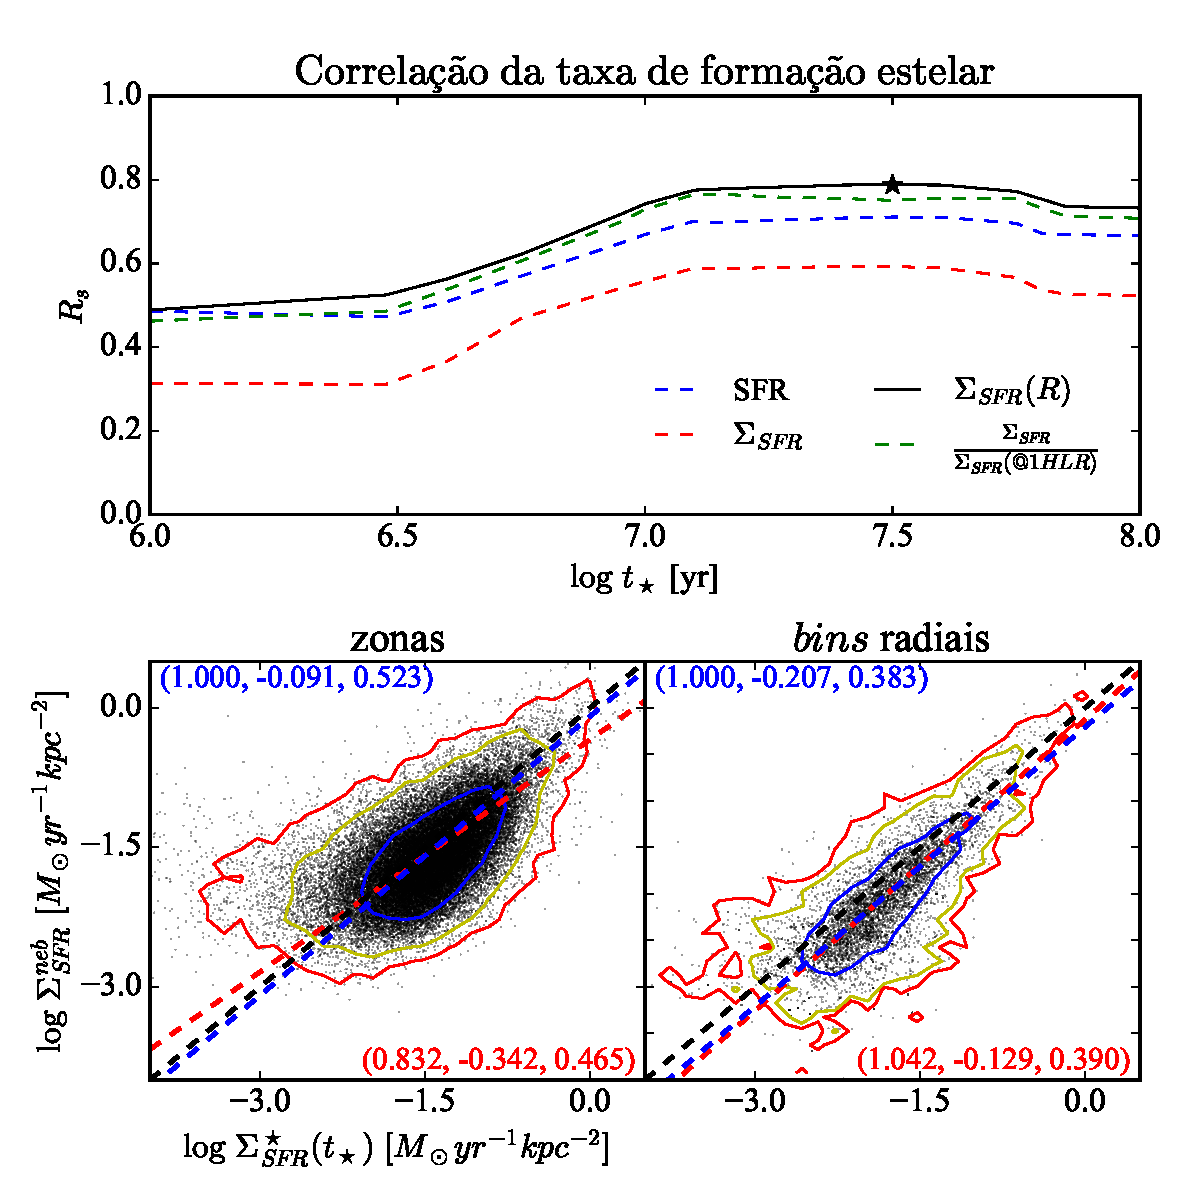
\includegraphics[scale=0.7, clip]{figuras/Rs_allSFR.pdf}
	\caption[Comparação entre as SFR.]
	{\emph{Painel superior}: o coeficiente de correlação de Spearmann entre as SFR para diferentes
$t_\star$. Para cada cor temos um tipo de cálculo de SFR e em linha preta contínua temos os valores
do coeficiente de Spearmann para os perfis radiais de $\Sigma_{\mathrm{SFR}}$, que possui o valor de
idade que utilizamos para ser nossa escala de tempo de formação estelar ($t_{SF})$ (marcado
por uma estrela preta). \emph{Painéis inferiores}: comparação entre as densidades superficiais da
SFR utilizando $t_\star = t_{SF} = 3.2 \times 10^7$ para zonas e {\em bins} radiais. Em cada painel
a linha pontilhada vermelha é o ajuste linear utlizando {\em OLS bisector}, em azul é o ajuste
forçando que o coeficiente angular seja 1 e em preto é a bissetriz ($x = y$). Os números no canto
inferior direito de cada painel temos o coeficiente angular, a interceptação da reta com o eixo
vertical, e a média quadráticas dos desvios em relação ao ajuste.}
	\label{fig:SFRsynvsneb}
\end{figure}

No primeiro painel da Fig. \ref{fig:SFRsynvsneb} vemos o que comentamos anteriormente sobre a pouca
variação do coeficiente de Spearmann no intervalo entre 12 e 56 milhões de anos. Apesar de que os
cortes definidos na Sec. \ref{sec:amostra:mask} com relação a idade e coeficiente de extinção
mínimos não estão aplicados, como mencionado anteriormente, o resultado não quase não altera muito
quando aplicamos os cortes. O que acontece com a aplicação da máscara é que a correlação para idades
mais baixas que nosso $t_{SF}$ escolhido aumentam e o desvio quadrático diminui. Nos paineis de
baixo vemos a correlação entre as densidades superficiais da taxa de formação estelar por zonas e
em {\em bins} radiais, calculando $\overline{\mathrm{SFR}_\star}(t_\star)$ utilizando $t_\star =
t_{SF} = 31.62$ milhões de anos. Juntamente ao ajuste {\em OLS} (em vermelho), adiciono um ajuste
forçando que o coeficiente angular seja 1 (em azul). A comparação utilizando os {\em bins} radiais
possuem desvio $rms$ 0.390 contra 0.465 quando comparamos o ajuste {\em OLS}.
 
Este procedimento de comparação foi feito também em \citet{Asari.etal.2007a}, no qual os autores
encontraram $t_{SF}$ igual a 25 milhões de anos, para 82302 galáxias do \SDSS. A síntese de
populações estelares foi realizada utilizando o \starlight, mas com uma diferente IMF. Apesar dessa
diferença a concordância entre os resultados é boa.

% \begin{figure}
% 	\centering
% 	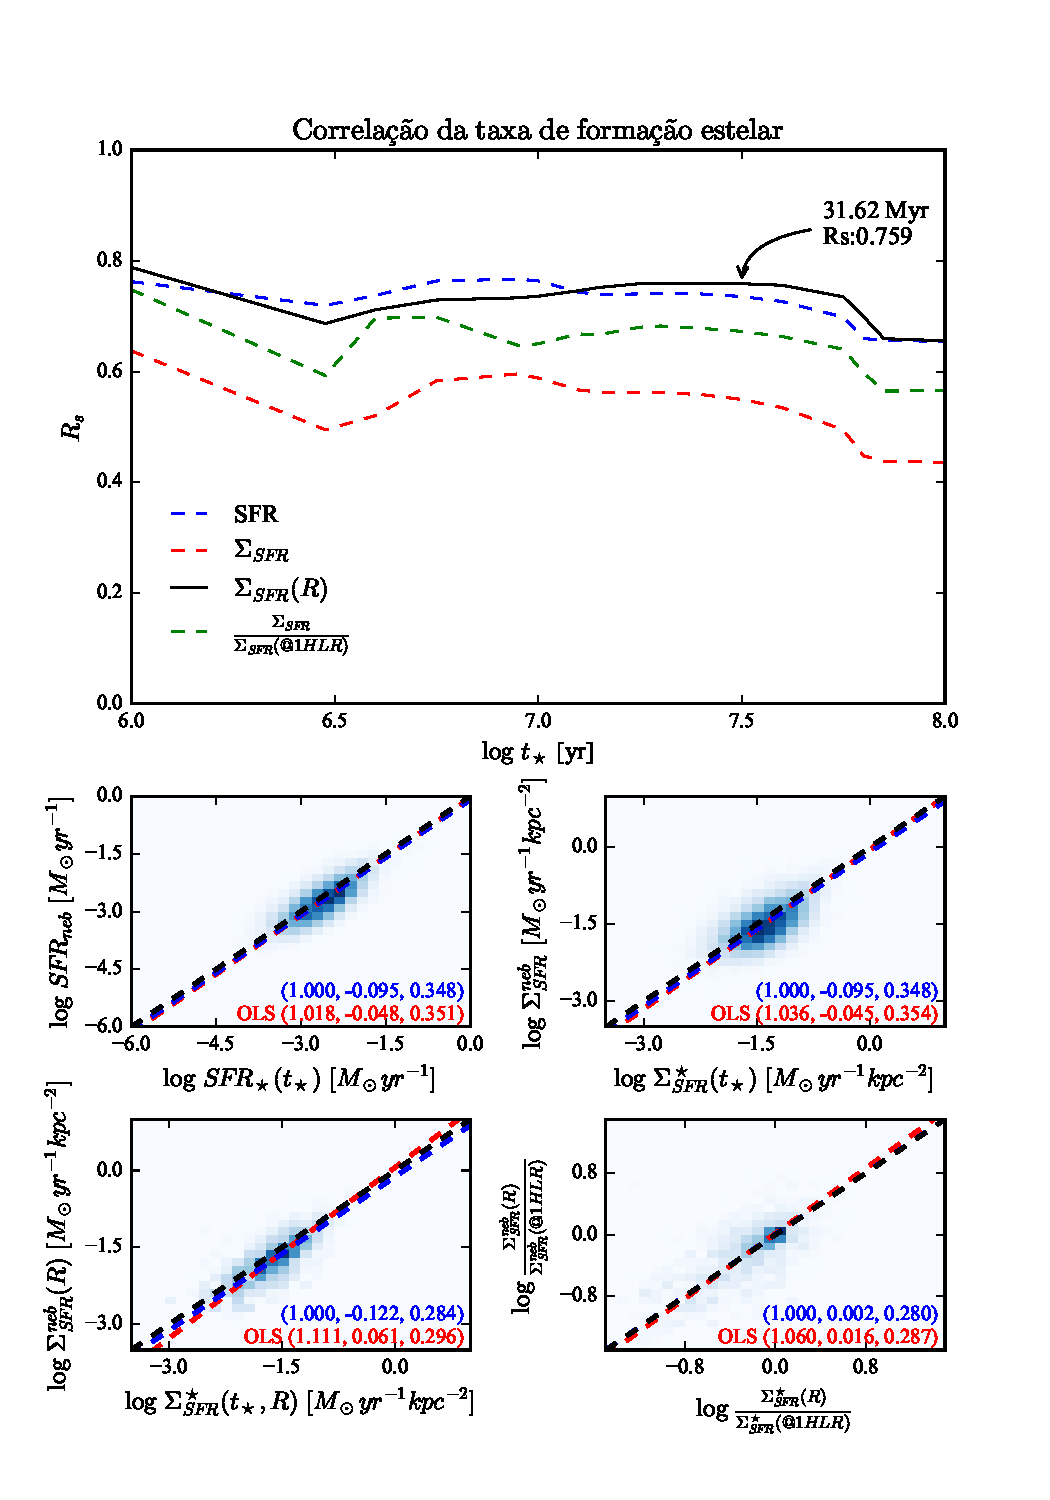
\includegraphics[scale=0.7, clip]{figuras/Rs_allSFR_cuts.pdf}
% 	\caption[Comparação entre as SFR após cortes.]
% 	{Igual a Fig. \ref{fig:SFRsynvsneb} mas com a aplicação dos cortes definidos em
% 	\ref{sec:amostra:mask}.}
% 	\label{fig:SFRsynvsneb_cuts}
% \end{figure}
% Figuras:
% - melhor comparação e ajuste

\section{Comparação entre os coeficientes de extinção}
\label{sec:synvsneb:tauv}

A síntese de populações estelares realizadas pelo \starlight adota o mesmo modelo de extinção por
poeira explicado em \ref{sec:emline:datacube:tauvneb}, onde todas as populações são atenuadas pelo
mesmo fator $e^{-\tau_\lambda}$. Essa simplificação contraria tanto evidências observacionais quanto
estudos teóricos, que caminham para um cenário onde populações mais jovens são mais atenuadas pela
poeira que populações mais velhas. \citet{Calzetti.etal.1994a} encontraram evidências diretas de que
a extinção em regiões \Hii é aproximadamente duas vezes maior do que a das estrelas ($\tauVS \sim
0.44 \tauVN$). \citet{Charlot.Fall.2000a} propõe um modelo onde populações jovens são atenuadas por
poeira na núvem de gás que a gerou e encontra que o coeficiente de extinção das {\em birth-clouds}
(BC) é cerca de 3 vezes maior que  do meio interestelar (ISM). \citet{Kreckel.etal.2013a} através de
dados de espectrografia de campo integrado do KINGFISH \citep{Kennicutt.etal.2011a} calculam a
densidade superficial de poeira dessas galáxias e chegam a conclusão que o coeficiente de extinção
derivados do contínuo estelar não correlaciona com a quantidade total de massa de poeira,
diferentemente daquele derivado do decremento Balmer.

Apesar do modelo de extinção ser o mesmo, o coeficiente calculado por cada um dos procedimentos é
diferente, como podemos ver através dos resultados da Fig. \ref{fig:tauVsynvsneb}. Esta figura
apresenta a comparação entre os coeficientes de extinção para zonas e também para os perfis radiais.
O coeficiente que vem do \starlight é calculado no processo de ajuste espectral, já o do decremento
de Balmer representa melhor as regiões onde existem os observáveis necessários para seu cálculo, ou
seja, regiões onde existam linhas de \Halpha e \Hbeta, portanto, regiões mais jovens. Verificamos
que a medida que vamos sendo mais exigentes com a fração de luz proveniente das populações jovens
($x_Y$), valor mínimo de $\tauVS$ e $\tauVN$, e distância radial de cada zona considerada na
comparação (ver Fig. \ref{fig:tauVsynvsnebMask}), as diferenças entre os dois coeficientes diminui,
iluminando um caminho que vamos nos aprofundar um pouco melhor no próximo capítulo e que pode nos
ajudar a um melhor entendimento do significado de $\tauVS$.

\begin{figure}
	\centering
	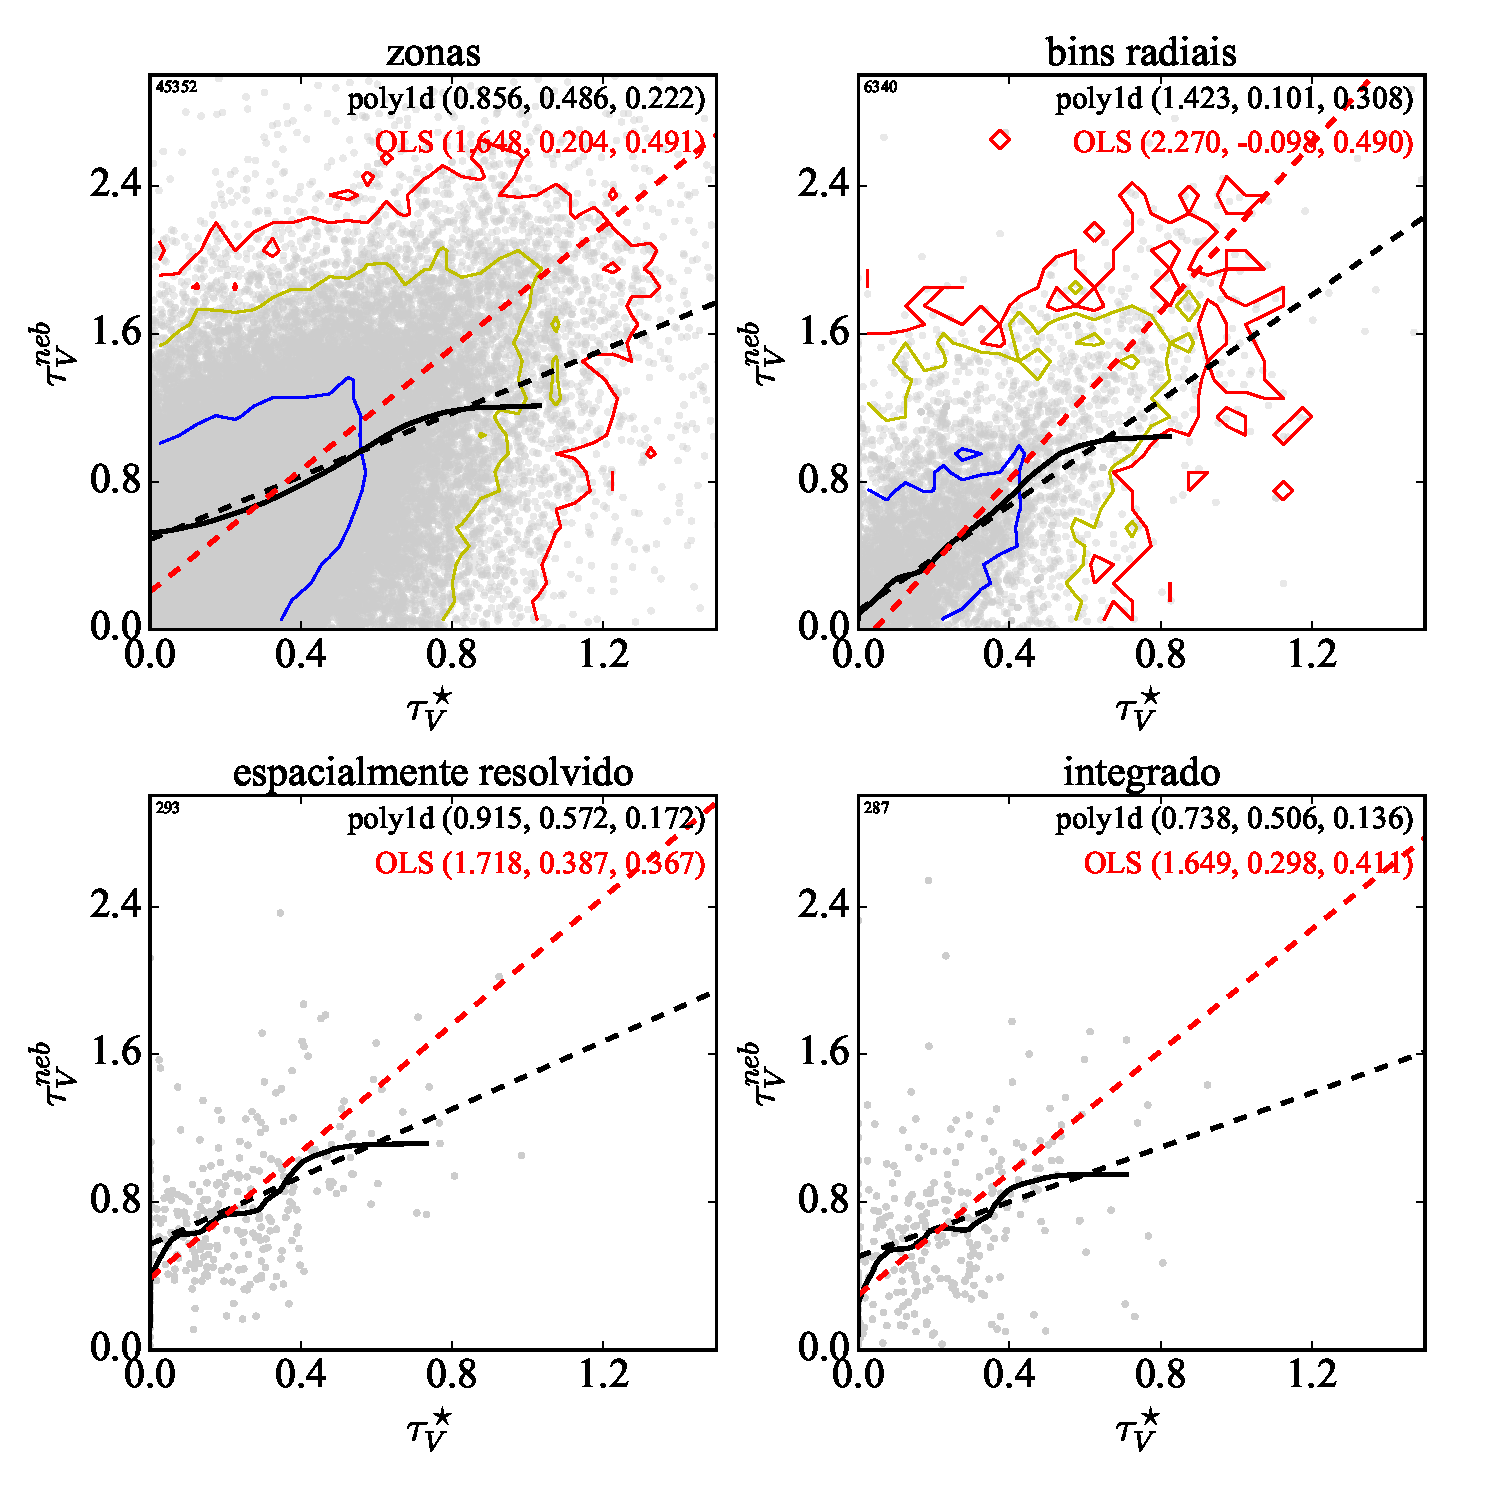
\includegraphics[width=0.99\textwidth]{figuras/CompareTauV.pdf}
	\caption[Comparação entre os coeficientes de extinção.] 
	{Comparação entre os coeficientes de extinção por poeira provenientes da síntese ($\tauVS$) e
do decremento de Balmer ($\tauVN$). Os contornos azul, amarelo e vermelho representam os
intervalos de confiança ($1\sigma$, $2\sigma$ e $3\sigma$). A linha preta representa a mediana e as linhas
pontilhadas representam o ajuste utilizando {\em OLS bisector} (vermelha) e mínimos quadrados
(preta). Como em todos os gráficos com ajustes lineares, em detalhe temos o coeficiente angular, a
interceptação da reta com o eixo vertical, e a média quadráticas dos desvios em relação a cada
ajuste. Este gráfico não possui a máscara da definição da amostra aplicada.}
	\label{fig:tauVsynvsneb}
\end{figure}

\begin{figure}
	\centering
	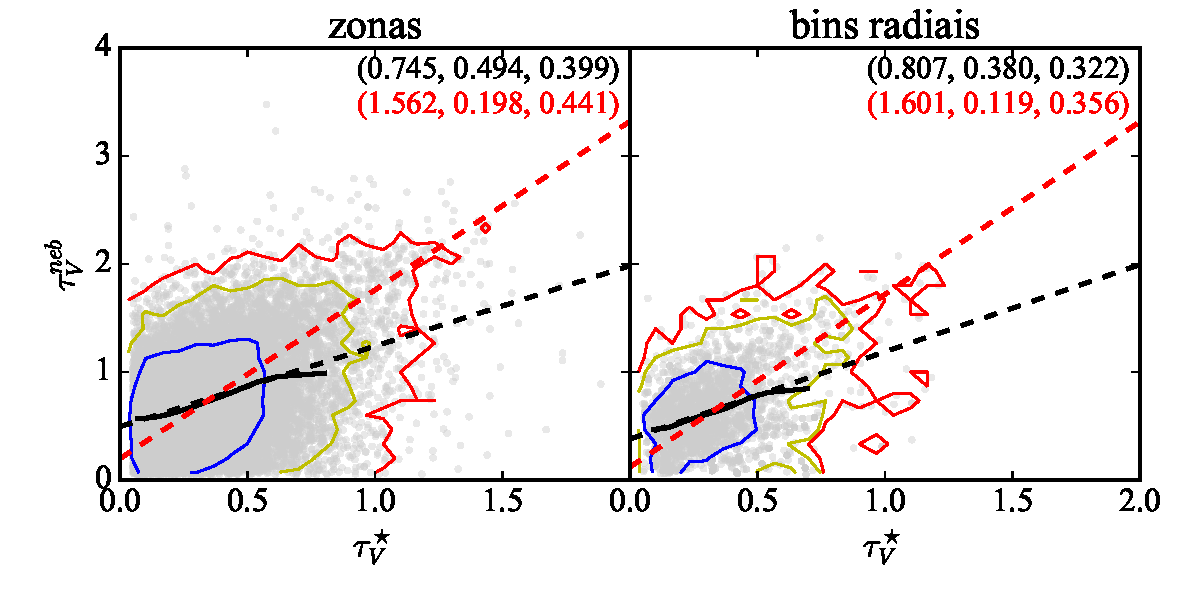
\includegraphics[width=0.99\textwidth]{figuras/CompareTauV_realsample.pdf}
	\caption[Comparação entre os coeficientes de extinção da amostra selecionada.]
	{Igual a Fig. \ref{fig:tauVsynvsneb} mas com a aplicação dos cortes definidos em
\ref{sec:amostra:mask}.} 
	\label{fig:tauVsynvsnebMask}
\end{figure}

% Figuras:
% - Exemplo de diferenças entre mapas de tau_V
% - comparação entre tauV
% - x_Y

\section{Comparação entre as metalicidades}
\label{sec:synvsneb:Z}

\subsection{Metais em galáxias - \meanM{\log Z_\star} e $\log\ (O/H)$}
\label{sec:synvsneb:ZemuZR}

Como citado em \ref{sec:emline:datacube:Zneb}, com a calibração de M13 temos a metalicidade nebular
para aquelas regiões aonde temos medidas para todas as linhas envolvidas no processo (\Hbeta, \oIII,
\Halpha e \nII). A metalicidade estelar para cada pixel (par $x,y$) é calculada segundo a equação:
\begin{equation}
 	\label{eq:logZmass}
 	\langle \log Z_\star \rangle_{M,xy} = 
	\frac{ \sum_{tZ} M_{\star,tZ,xy} \times \log\ Z}{
	\sum_{tZ} M_{\star,tZ,xy} }.
\end{equation}
\noindent onde $M_{\star,tZ,xy}$ representa a massa em estrelas com idade $t$ e metalicidade $Z$ no
pixel $xy$. 

Na Fig. \ref{fig:compareZR} vemos em detalhe a comparação entre as metalicidades estelar e nebular
para os perfis radiais e das galáxias de nossa amostra. A comparação entre essas duas propriedades
deve ser analisada com cuidado, porque estamos tratando de coisas bem diferentes derivadas de
maneira completamente diferente, todavia a correlação existe e já foi identificada por diversos
artigos \citep{CidFernandes.etal.2005a, Gallazzi.etal.2005a, CidFernandes.etal.2007a,
Asari.etal.2007a}. \citet{Stasinska.etal.2006a} enfatiza que esse método de derivação de
metalicidade nebular utilizando {\em strong-line methods} são calibrados geralmente em gigantes
regiões \Hii, portanto ainda são necessários estudos sobre os gradientes de metalicidades dentro de
galáxias. Ainda sim, vejo uma boa correlação entre as duas medidas. Os valores para zonas possuem
muito espalhamento, mas quando verificamos os valores os perfis radiais (e também os valores
integrados, embora aqui não demonstrados) vemos que existe uma boa correlação entre as duas com um
espalhamento pequeno (em todos os {\em bins} menor que 0.2 dex). Vemos também que temos uma
tendência para que populações na parte mais interna do disco possuam metalicidades mais altas que
nas partes externas. Essa discussão é muito interessante e precisa ser muito desenvolvida, mas não
faz parte dessa nossa primeira etapa. Entretanto, a conversão de poeira para gás deve ser dependente
de metalicidade, portanto, o tema surgirá nas próximas etapas deste trabalho.

\begin{figure}
	\centering
	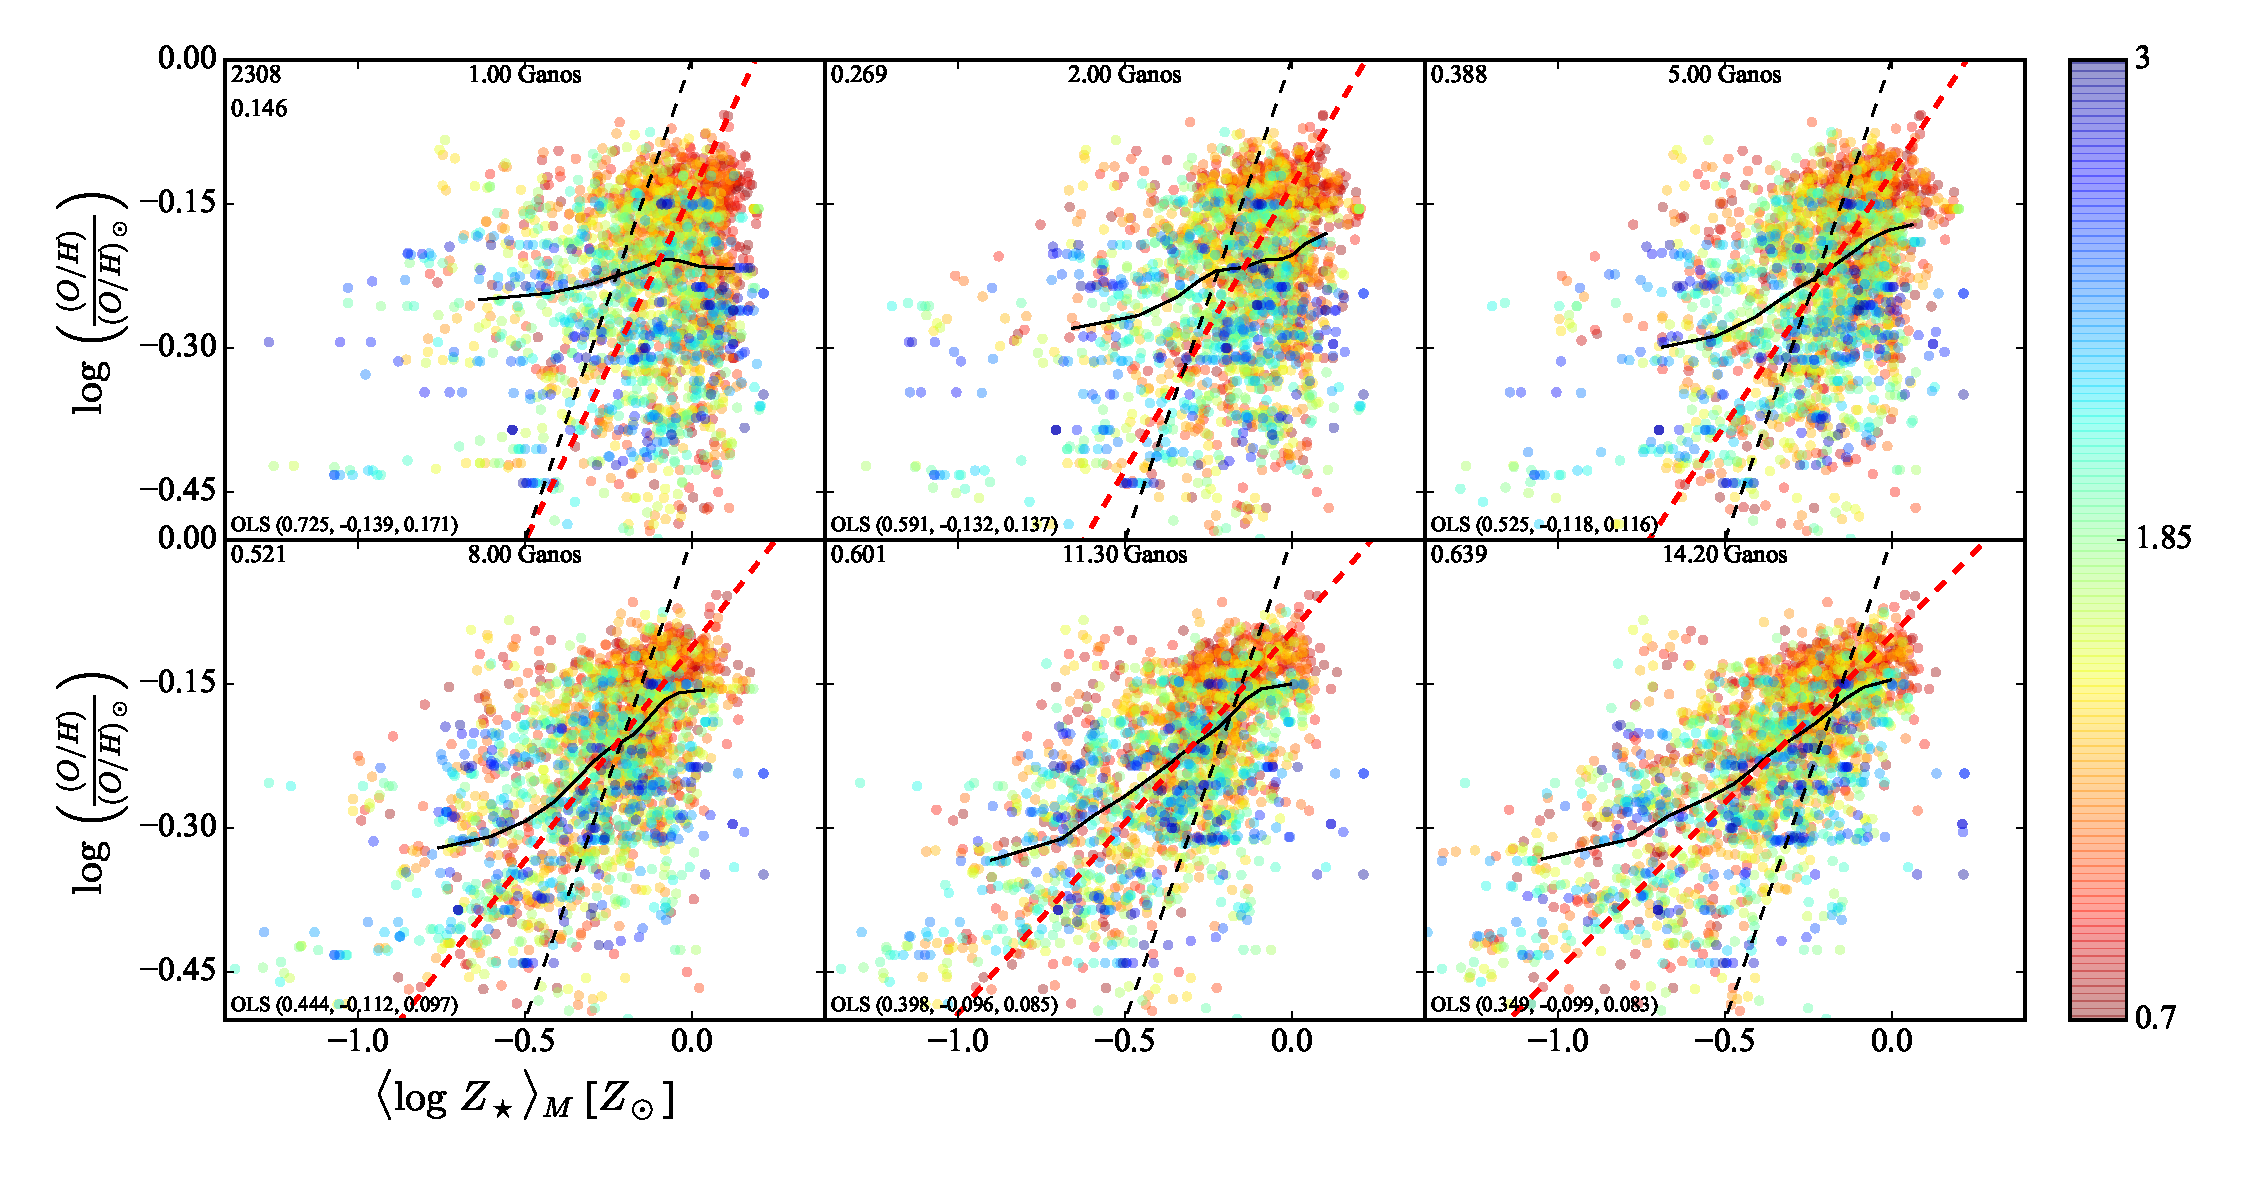
\includegraphics[width=0.99\textwidth]{figuras/CompareZR.pdf}
	\caption[\meanM{\log Z_\star} vs. $\log\ (O/H)$ - perfis radiais]
	{Comparação entre a metalicidade do gás ($\log\ (O/H)$) e metalicidade média das populações
estelares (\meanM{\log Z_\star}) calculada para diferentes intervalos de tempo (1, 2, 5, 8, 11.3 e
14.2 bilhões de anos). Em cada gráfico em vermelho o {\em OLS bisector} e a bissetriz em negro.
Novamente em detalhe o coeficiente angular, a interceptação da reta com o eixo vertical, e a média
quadráticas dos desvios em relação ao ajuste.}
	\label{fig:compareZR}
\end{figure}

% \begin{figure}
% 	\centering
% 	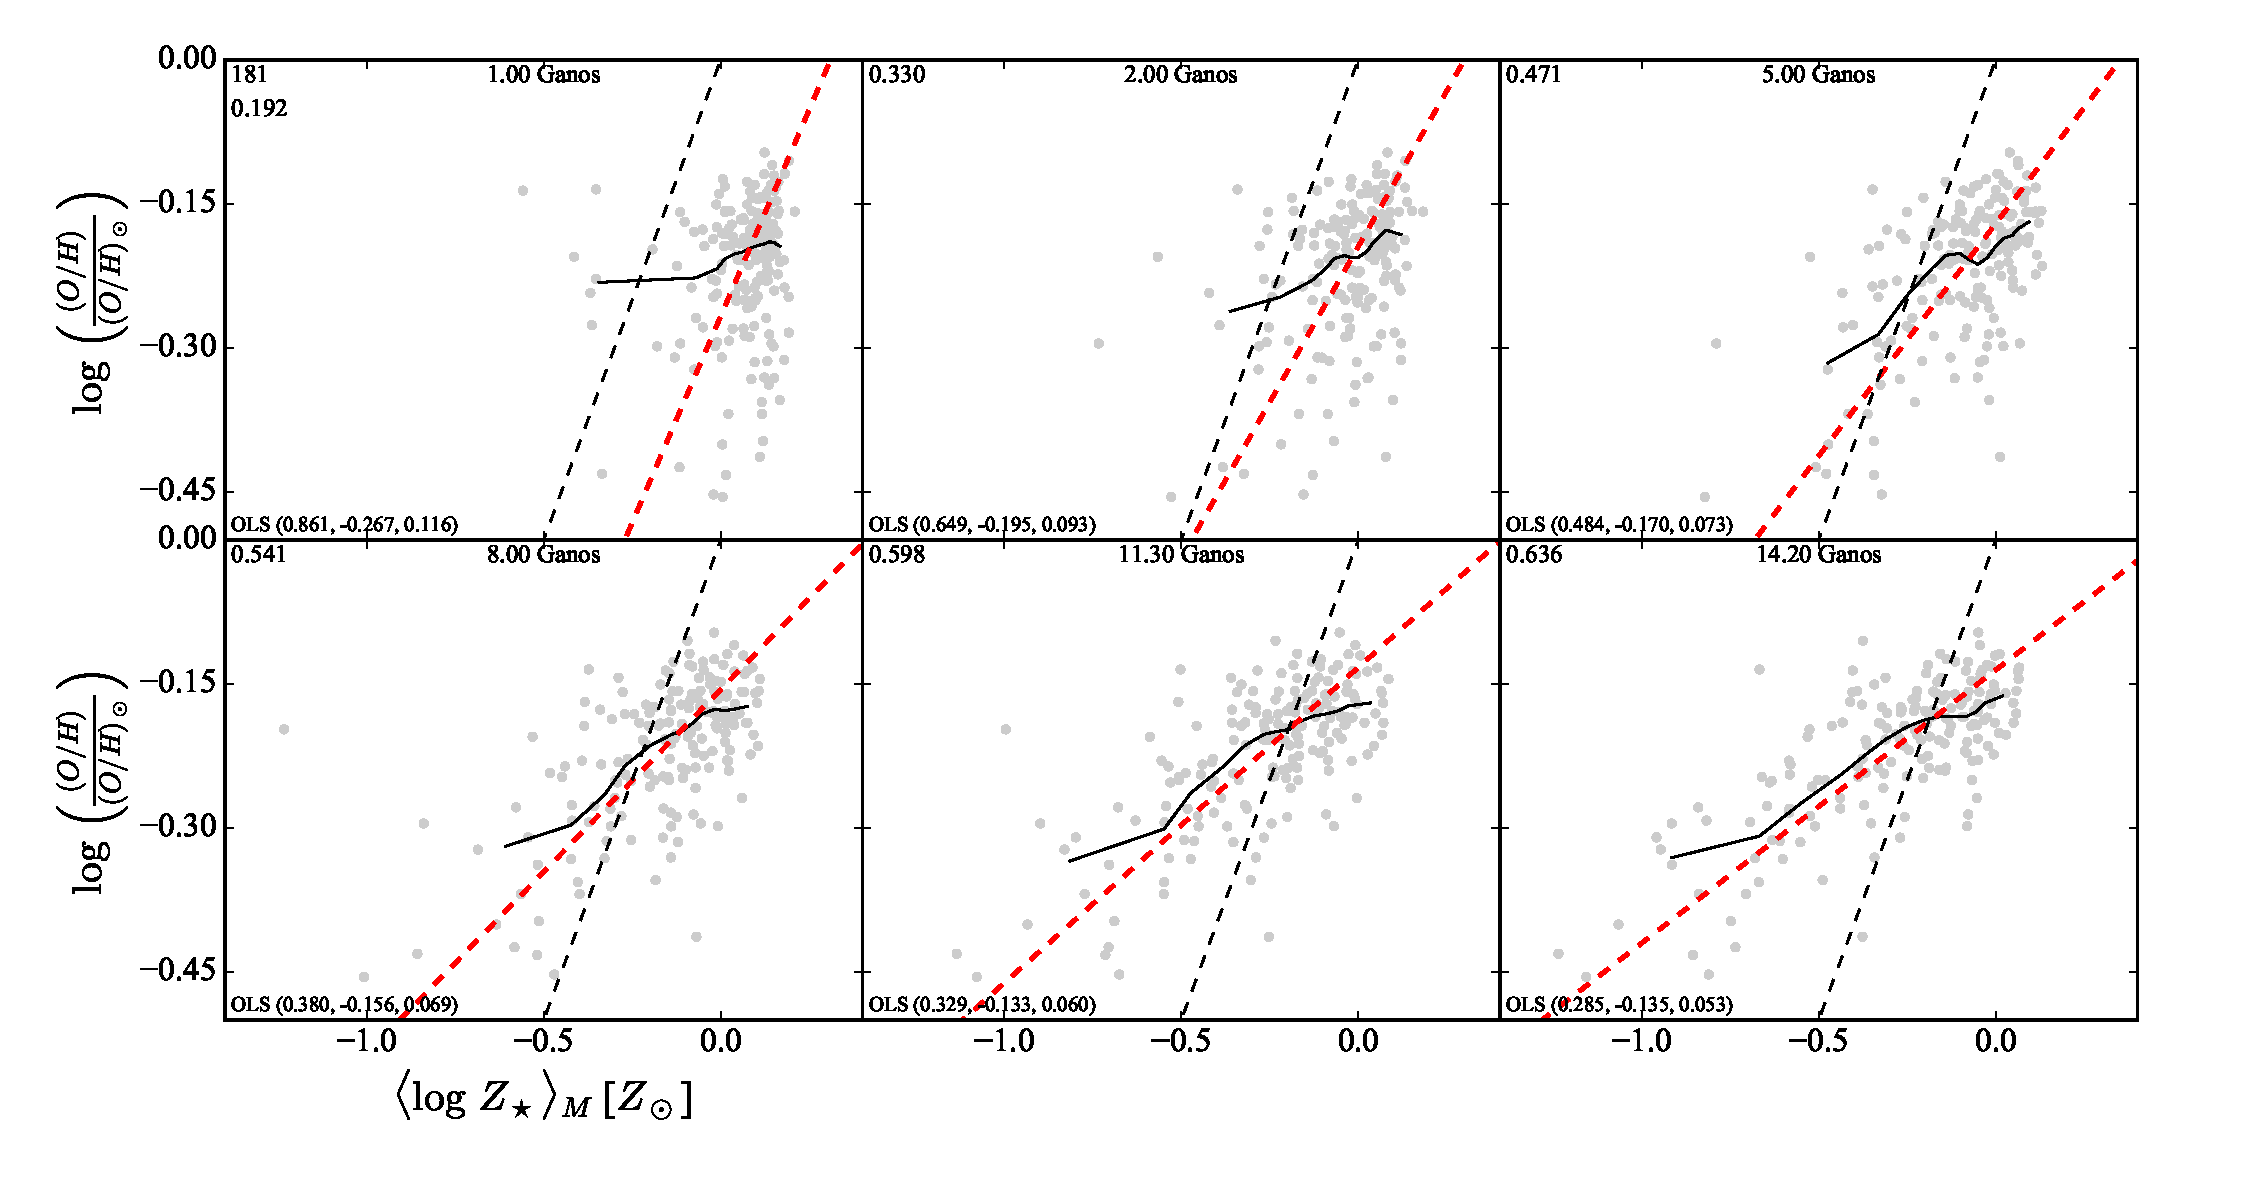
\includegraphics[width=0.99\textwidth]{figuras/CompareZint.pdf}
% 	\caption[\meanM{\log Z_\star} vs $\log\ (O/H)$ - galáxias integradas]
% 	{Igual a Fig. \ref{fig:compareZR} mas com um ponto por galáxia (valores integrados).}
% 	\label{fig:compareZint}
% \end{figure}

\subsection{Artigo - Insights on the Stellar Mass-Metallicity Relation from the CALIFA Survey.}

No artigo de \citet{GonzalezDelgado.etal.2014b} (GD14 daqui em diante), cuja versão completa está no
apêndice \ref{apendice:GDetal2014b}, analisamos a relação entre massa estelar ($M_\star$ - efeitos
globais) e a densidade superficial de massa estelar ($\mu_\star$ - efeitos locais) com a
metalicidade estelar ($\meanM{\log Z_\star}$) de uma amostra de 300 galáxias do CALIFA de todos os
tipos morfológicos (desde E a Sd). \citet{Tremonti.etal.2004a} investigam a mesma relação, embora
para a metalicidade do gás ($\ZN$) e apenas para galáxias SF. Essa relação é conhecida como relação
massa-metalicidade ({\em mass-metallicity relation} - MZR). Verificamos que a MZR estelar é mais
inclinada e se estende em um intervalo muito maior comparando com aquela utilizando a metalicidade
do gás pois esta última nos fornece informações sobre o estado atual do gás e a primeira, sobre toda
a história de formação estelar da galáxia. 

\citet{Sanchez.etal.2013a} analisa essa relação para $\sim 3000$ regiões \Hii mapeadas em 150
galáxias do CALIFA. Comparando nossos resultados com os obtidos por \citeauthor{Sanchez.etal.2013a}
(Fig. 2b em GD14) nestas regiões vemos que eles se distanciam conforme $M_\star$ diminui.
Após calculamos a metalicidade estelar considerando apenas populações jovens ($t_\star\ \leq$ 2
bilhões de anos) vemos que o resultado se aproxima melhor da tendência para as regiões \Hii.

Utilizando nossa amostra, vemos na Fig. \ref{fig:ZstarvsZneb} a relação entre a densidade
superficial de massa estelar e a metalicidade nos três painéis de cima (zonas, anéis elípticos e
galáxias integradas) e, na mesma sequência, temos a comparação entre a metalicidade nebular e
estelar. Em cada gráfico aparecem as medianas para as metalicidades estelares calculadas para
diferentes intervalos de idades (de 1 a 14 bilhões de anos) de modo a ilustrar a sequência de
evolução química inferida a partir da síntese. A figura nos mostra que para mesmos valores de
$\mu_\star$ a metalicidade estelar é mais alta para as estrelas mais jovens, o que parece ser um
resultado coerente imaginando que o meio onde as novas estrelas nascem vai enriquecendo quimicamente
com o passar do tempo, fazendo com que novas estrelas tenham maior metalicidade. A metalicidade
nebular (marcada com uma linha tracejada preta) parece ser muito menos sensível às regiões mais
massivas do que a metalicidade estelar. \citet{Zahid.etal.2014a}, analisando galáxias com $z
\lesssim 1.6$, argumentam que esse achatamento acontece quando $M_\star \gg M_{\mathrm{gas}}$
($f_{\mathrm{gas}} \to 0$; ver Eq. \ref{eq:fgas}), assim a quantidade de oxigênio presa dentro das
estrelas ({\em lock-up fraction}) de baixa massa é da ordem daquela produzida pelas estrelas de alta
massa. Os modelos de evolução química evoluíram bastante nos últimos anos \citep[e.g.,
][]{Lilly.etal.2013a, Peng.Maiolino.2014a, Ascasibar.etal.2015a, Peng.Maiolino.Cochrane.2015a} e
esperamos que logo tenhamos melhores resultados nessa área. O tema é muito interessante e tem muito
ainda a ser explorado, principalmente quanto aos efeitos locais, quando analisamos esta relação
internamente nas galáxias e seus efeitos em parâmetros globais. Sobre o painel abaixo, o que vemos é
que a variação da metalicidade estelar é muito maior do que a nebular e a correlação entre ambas vai
aumentando à medida que vamos de zonas para galáxias integradas. O painel inferior central condensa
todos os painéis da Fig. \ref{fig:compareZR}.

\begin{figure}
	\centering
	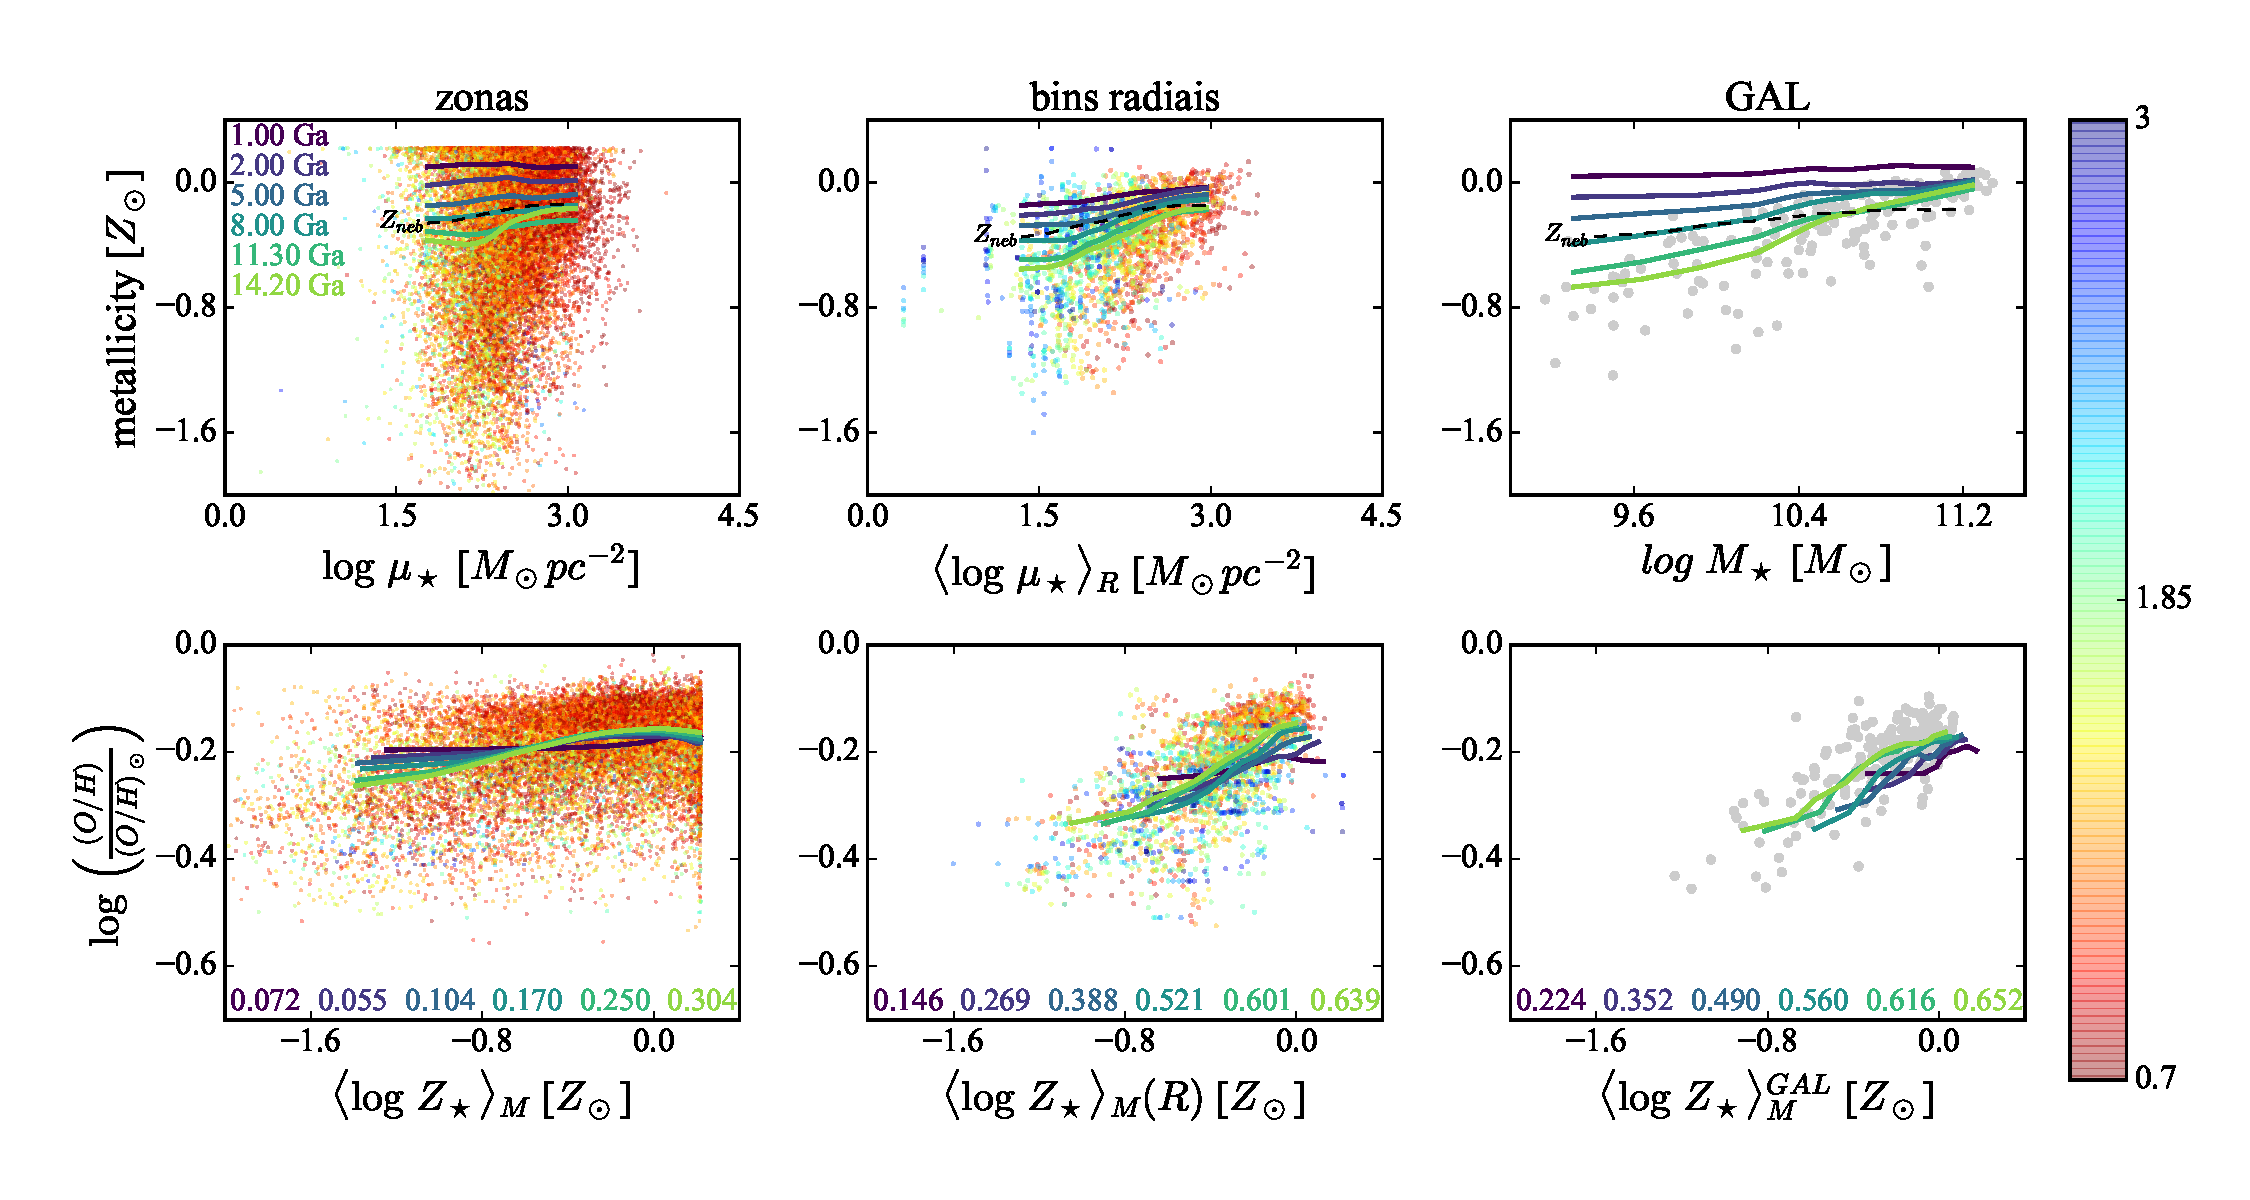
\includegraphics[width=0.99\textwidth]{figuras/stellar_muZR_realsample.pdf}
	\caption[Relação $\mu$ZR e comparação entre as metalicidades.]
	{Relação $\mu$ZR para zonas ({\em painel a}), {\em bins} radiais ({\em painel b}) e galáxias
integradas ({\em painel c}). Os pontos desenhados em cada gráfico representam $\meanM{\log Z_\star}$
calculado para todas as populações com distintas idades, coloridos pela distância radial (barra de
cores em HLR). Cada gráfico possui a mediana da distribuição de $\meanM{\log Z_\star}$ para
diferentes intervalos de população ($t_\star \leq$ 1, 2, 5, 8, 11.3 e 14.2 bilhões de anos), além
da mediana para $\ZN$ ($\log(O/H)$). Comparação $\meanM{\log Z_\star}$ e
$\ZN$ seguindo a mesma configuração acima (zonas ({\em painel d}), raio ({\em painel e}) e
integrados ({\em painel f})) com as medianas por diferentes intervalos de população no cálculo de
$\meanM{\log Z_\star}$ também. Seguindo o mesmo padrão de cores para as medianas, abaixo de cada
gráfico vemos o coeficiente de correlação de Spearmann entre $\meanM{\log Z_\star}$ e $\ZN$.}
	\label{fig:ZstarvsZneb}
\end{figure}

\subsection{Artigo - The CALIFA Survey across the Hubble sequence. Spatially resolved stellar
population properties in galaxies}

Durante o tempo que estive no IAA tive participação em dois artigos. O segundo deles
\citep{GonzalezDelgado.etal.2015a} (em anexo, \ref{apendice:GDetal2015a}) é um artigo onde
resolvemos espacialmente as propriedes estelares baseados na síntese com o \starlight para 300
galáxias do \CAL entre todos os tipos morfológicos. Verificamos que as galáxias mais massivas são
mais densas, velhas, mais ricas em metais e menos extinguídas por poeira. Discutimos algumas como as
propriedades se comportam em partes distintas da galáxia (bojo e disco) e o quanto essas
propriedades variam quando dividimos em classes de massa, idade e tipo morfológico. Galáxias do tipo
Sb-Sbc possuem gradientes de \meanM{\log Z_\star} compatíveis com aqueles medidos para a Via Láctea.
Galáxias tipo Sc possuem gradientes mais planos, nos mostrando que a evolução química do disco
contribui bastante com a evolução química das galáxias desta classe morfológica. Em uma visão geral,
concluímos que o processo de parada de formação estelar\footnote{Geralmente conhecido como {\em
quenching}.} é geralmente independente da massa total da galáxia, enquanto metalicidade e a
estrutura física da galáxia são influenciadas por processos que são dependentes da massa.

%Estudos recentes apontam valores similares para o tempo de depleção do gás \citep[e.g., ][ver tabela 5 e
%referências.]{Leroy.etal.2013a}. As galáxias mais massivas completaram seu enriquecimento químico a
%muitas eras atrás, com a história de formação estelar geralmente aproximanda a um único largo broto
%de formação estelar. Hoje, as galáxias menos massivas são aquelas que possuem maior atividade de
%formação estelar. Esse fenômeno é conhecido como {\em Downsizing} \myojo{blue}{REFS?}.

% Quando calculamos a metalicidade média das populações jovens das galáxias, estamos olhando para as
% populações estelares de galáxias menos massivas, mais jovens e com atividade de formação estelar
% intensa, portanto com um interva

% Figuras:
% - comparação entre metalicidades

%% End of this chapter
